% PhyriadFG — frame-generation pipeline: how the intermediate frame I_t is born
% Build:  pdflatex phyriadfg_pipeline.tex   ->  phyriadfg_pipeline.pdf
% Raster: pdftoppm -png -r 200 phyriadfg_pipeline.pdf phyriadfg_pipeline
\documentclass[border=10pt]{standalone}
\usepackage[T1]{fontenc}
\usepackage{amsmath}
\usepackage{xcolor}
\usepackage{tikz}
\usetikzlibrary{arrows.meta,positioning,fit,backgrounds,calc}

\definecolor{Lcapture}{HTML}{1F77B4}
\definecolor{Lflow}{HTML}{17BECF}
\definecolor{Lwarp}{HTML}{FF7F0E}
\definecolor{Lblend}{HTML}{D62728}
\definecolor{Lquality}{HTML}{2CA02C}
\definecolor{Lpresent}{HTML}{9467BD}
\definecolor{Lsync}{HTML}{E377C2}

\begin{document}
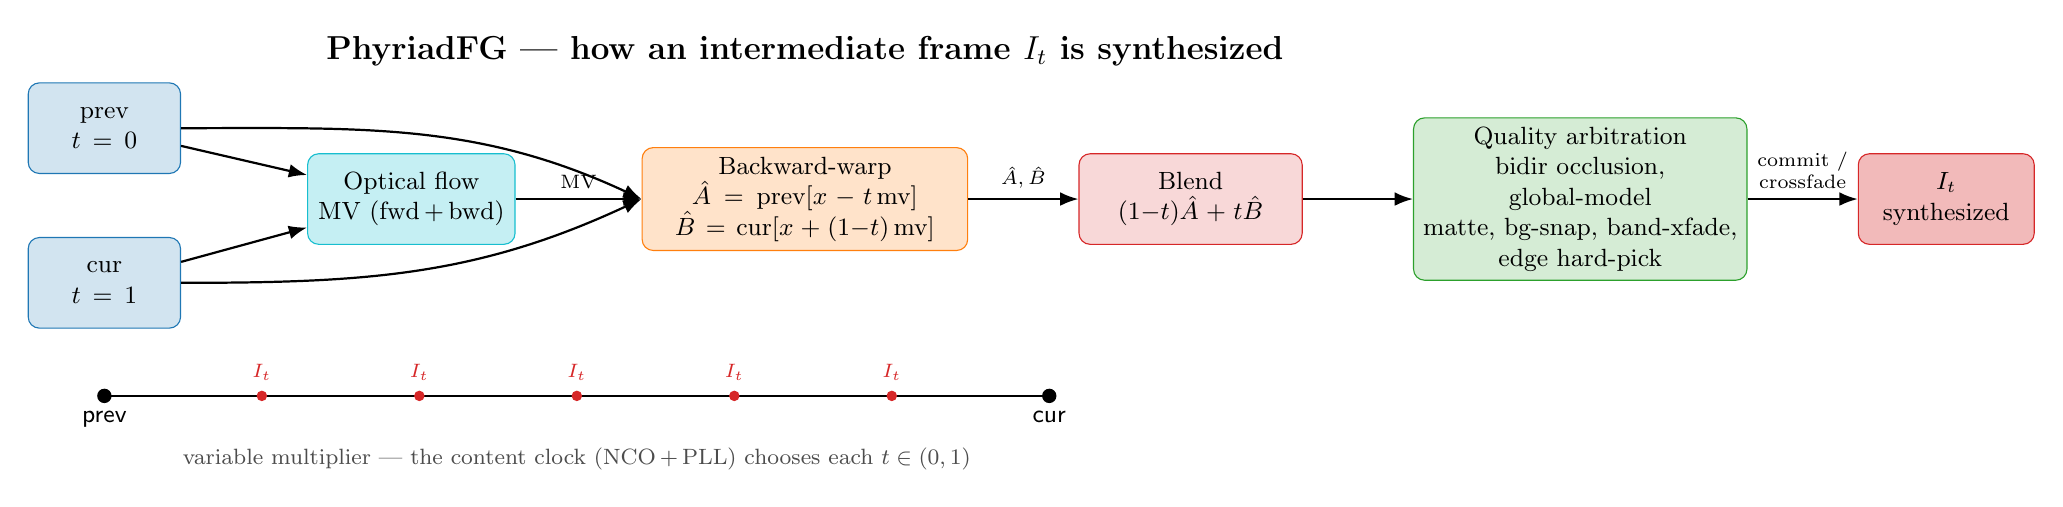
\begin{tikzpicture}[
  font=\sffamily, >=Latex,
  box/.style={draw, rounded corners, minimum height=1.15cm, align=center, font=\small},
  elab/.style={midway, above, font=\scriptsize, align=center},
]

% ── inputs: two real frames ──────────────────────────────────────────
\node[box, fill=Lcapture!20, draw=Lcapture, text width=1.7cm] (A) {prev\\$t=0$};
\node[box, fill=Lcapture!20, draw=Lcapture, text width=1.7cm, below=8mm of A] (B) {cur\\$t=1$};

% ── optical flow ─────────────────────────────────────────────────────
\node[box, fill=Lflow!25, draw=Lflow, right=16mm of A, yshift=-9mm, text width=2.4cm] (fl)
  {Optical flow\\MV (fwd\,+\,bwd)};

% ── backward warp ────────────────────────────────────────────────────
\node[box, fill=Lwarp!22, draw=Lwarp, right=16mm of fl, text width=3.9cm] (wp)
  {Backward-warp\\$\hat A=\text{prev}[x-t\,\text{mv}]$\\$\hat B=\text{cur}[x+(1{-}t)\,\text{mv}]$};

% ── blend ────────────────────────────────────────────────────────────
\node[box, fill=Lblend!18, draw=Lblend, right=14mm of wp, text width=2.6cm] (bl)
  {Blend\\$(1{-}t)\hat A + t\hat B$};

% ── quality arbitration ──────────────────────────────────────────────
\node[box, fill=Lquality!20, draw=Lquality, right=14mm of bl, text width=4.0cm] (q)
  {Quality arbitration\\bidir occlusion, global-model\\matte, bg-snap, band-xfade,\\edge hard-pick};

% ── output ───────────────────────────────────────────────────────────
\node[box, fill=Lblend!32, draw=Lblend, right=14mm of q, text width=2.0cm] (it)
  {$I_t$\\synthesized};

% edges
\draw[->, thick] (A) -- (fl); \draw[->, thick] (B) -- (fl);
\draw[->, thick] (A.east) to[out=0,in=155] (wp.west);
\draw[->, thick] (B.east) to[out=0,in=205] (wp.west);
\draw[->, thick] (fl) -- (wp) node[elab]{MV};
\draw[->, thick] (wp) -- (bl) node[elab]{$\hat A,\hat B$};
\draw[->, thick] (bl) -- (q);
\draw[->, thick] (q)  -- (it) node[elab]{commit /\\crossfade};

% ── timeline (variable multiplier, content clock chooses t) ──────────
\begin{scope}[yshift=-34mm]
  \draw[thick] (0,0) -- (12,0);
  \fill (0,0) circle (2.6pt); \fill (12,0) circle (2.6pt);
  \node[below=2pt] at (0,0) {\small prev};
  \node[below=2pt] at (12,0) {\small cur};
  \foreach \x in {2.0,4.0,6.0,8.0,10.0}{
     \fill[Lblend] (\x,0) circle (1.9pt);
     \node[above=2pt, Lblend, font=\scriptsize] at (\x,0) {$I_t$};
  }
  \node[font=\footnotesize, text=black!70] at (6,-0.8)
    {variable multiplier --- the content clock (NCO\,+\,PLL) chooses each $t \in (0,1)$};
\end{scope}

% ── caption ──────────────────────────────────────────────────────────
\node[font=\large\bfseries, above=9mm of wp, anchor=south]
  {PhyriadFG --- how an intermediate frame $I_t$ is synthesized};

\end{tikzpicture}
\end{document}
